% Provisional manuscript revision, 2 November 2026. Compile with pdfLaTeX + BibTeX.
% Counts come from generated/counts.tex and figures from figures/, both produced by
% review-paper/scripts/make_figures.py and make_tables.py from the replayable CSV records.
% Remaining [Author input] items need the authors; do not submit while any remain.
\documentclass[journal]{IEEEtran}
\usepackage[T1]{fontenc}
\usepackage[utf8]{inputenc}
\usepackage{cite}
\usepackage{amsmath,amssymb}
\usepackage{graphicx}
\usepackage{booktabs,tabularx,array}
\usepackage[hidelinks]{hyperref}
\graphicspath{{figures/}}
\newcommand{\authorinput}[1]{\par\noindent\textit{[Author input required: #1]}\par\smallskip}
\newcolumntype{Y}{>{\raggedright\arraybackslash}X}
% Generated by scripts/make_tables.py
\newcommand{\nIdentified}{6,683}
\newcommand{\nOpenAlex}{6,250}
\newcommand{\nCrossref}{400}
\newcommand{\nSeeds}{33}
\newcommand{\nDuplicates}{1,098}
\newcommand{\nScreened}{5,585}
\newcommand{\nTAExcluded}{4,392}
\newcommand{\nTABackground}{406}
\newcommand{\nSought}{787}
\newcommand{\nNotRetrieved}{568}
\newcommand{\nAssessed}{219}
\newcommand{\nFTBackground}{11}
\newcommand{\nIncluded}{157}
\newcommand{\nIncludedReports}{170}
\newcommand{\nSecondary}{13}
\newcommand{\nFTExcluded}{36}
\newcommand{\nExFTOne}{3}
\newcommand{\nExFTTwo}{2}
\newcommand{\nExFTThree}{5}
\newcommand{\nExFTFour}{15}
\newcommand{\nExFTFive}{3}
\newcommand{\nExFTSix}{23}
\newcommand{\nAnyOne}{43}
\newcommand{\nPrimOne}{19}
\newcommand{\nAnyTwo}{16}
\newcommand{\nPrimTwo}{6}
\newcommand{\nAnyThree}{99}
\newcommand{\nPrimThree}{70}
\newcommand{\nAnyFour}{29}
\newcommand{\nPrimFour}{13}
\newcommand{\nAnyFive}{25}
\newcommand{\nPrimFive}{11}
\newcommand{\nAnySix}{12}
\newcommand{\nPrimSix}{7}
\newcommand{\nAnySeven}{24}
\newcommand{\nPrimSeven}{12}
\newcommand{\nAnyEight}{50}
\newcommand{\nPrimEight}{19}
\newcommand{\nEnergy}{21}
\newcommand{\nManufacturing}{105}
\newcommand{\nInfra}{27}
\newcommand{\nOther}{4}
\newcommand{\nBench}{98}
\newcommand{\nIndOffline}{46}
\newcommand{\nField}{8}
\newcommand{\nDeployed}{4}
\newcommand{\nHumanExp}{1}
\newcommand{\nGuarFS}{4}
\newcommand{\nGuarEOP}{16}
\newcommand{\nGuarNone}{137}
\newcommand{\nHumNone}{116}
\newcommand{\nHumRec}{11}
\newcommand{\nHumDes}{23}
\newcommand{\nHumEval}{7}
\newcommand{\nShiftNatural}{74}
\newcommand{\nShiftSynthetic}{35}
\newcommand{\nShiftBoth}{10}
\newcommand{\nRecent}{105}
\newcommand{\pctRecent}{67}
\newcommand{\pctEnergy}{13}
\newcommand{\pctBench}{62}
\newcommand{\nPublicArtifacts}{41}
\newcommand{\nMVTec}{48}
\newcommand{\nVisA}{19}
\newcommand{\nRestricted}{24}
\newcommand{\nAUROCEval}{53}
\newcommand{\nCalibEval}{12}
\newcommand{\nRiskCoverage}{5}
\newcommand{\nFalseAlarm}{7}
\newcommand{\nVLM}{25}
\newcommand{\nThreeNatural}{71}
\newcommand{\nThreeSynthetic}{26}

% Generated by scripts/make_tables.py
\newcommand{\citeOne}{\cite{nash2022deep,alqahtani2026robust,estermann2026unsupervised,rintrawong2026coverage,sarkar2026baypranometa,wang2022automated,khandagale2026dasformer,gohel2026interpretable,kibet2026self,corredor2026interpretable,khandagale2026meta,kompanets2026evaluation,kang2019contact,kyem2026multi,rozanec2023active,malihi2026quantitative,wu2026chips,klos2025super,prakash2026hybrid,mueez2026vision,ghasemlou2026cross,thakur2024deep,sajedi2020model,plevris2025assessing,li2025efficient,liang2021pushing,liang2020deep,patel2026precision,avramov2026synthetic,mikayilov2025development,li2026beyond,gramelt2025interactive,liu2026insightx,niu2024learning,jiang2026anomalyclaw,bence2026yolov,abbassi2024trimming,chen2025attack,cao2026robust,aqeel2025robust,krumpl2026iconic,han2026sparc,yang2026saferestore}}
\newcommand{\citeTwo}{\cite{estievenart2025risk,alqahtani2026robust,estermann2026unsupervised,rozanec2023active,wu2026chips,prakash2026hybrid,mueez2026vision,sun2026icme,kinalioglu2026risk,mistry2026from,frittoli2021deep,jia2026adaptive,lo2026semantic,deng2026distribution,zia2026learning,yang2026saferestore}}
\newcommand{\citeThree}{\cite{nash2022deep,estievenart2025risk,hecklerkram2026the,hoang2026supervised,ndjoko2026automated,kashiani2025roads,sundaravadivel2026adaptive,khandagale2026dasformer,gohel2026interpretable,kibet2026self,khandagale2026meta,kyem2026multi,jiang2021vision,chang2024rad,mueez2026vision,ghasemlou2026cross,sun2026icme,tang2023autonomous,li2025efficient,patel2026precision,xie2024iad,poniatowski2025domain,johansson2026poisoning,jeong2025domain,alvarez2026foundation,mu2025nexvitad,kinalioglu2026risk,liang2026open,reginald2026plant,trinh2024multiple,dmytro2025synthetic,wu2026hdsi,mistry2026from,durmaz2023microstructure,he2026self,leyendecker2023study,hecklerkram2026detecting,mondal2025class,frittoli2021deep,santos2022domain,avramov2026synthetic,li2023building,bartczak2026dataset,mikayilov2025development,amoshie2026domain,hecklerkram2025from,thota2020introducing,xie2024investigation,asadi2026cracksegflow,jia2026adaptive,wang2026cross,kemeter2024towards,chauhan2026acvrl,demircantureyen2026exploring,prajapati2025generative,yosifov2026directional,jaziri2024designing,tabassum2024adapting,li2026beyond,chen2026aranet,asadi2026fms,song2024source,cordier2022improving,jiang2026anomalyclaw,deng2026maf,bence2026yolov,abbassi2024trimming,chen2025attack,wu2026hid,wang2025lightweight,cao2023anomaly,zia2026learning,ding2022catching,wang2025distribution,wang2023robustness,lo2022adversarially,weatherly2026rethinking,cheng2024rad,mirzaei2024killing,lin2025exploring,moradi2025rddpm,nafez2025patchguard,chen2022domain,ilyas2026enhancing,bugarin2024unveiling,yu2025noise,krumpl2026iconic,deng2026global,pezze2025continual,barusco2025memory,yao2023explicit,baitieva2025beyond,lei2025adapted,bao2023miad,han2026sparc,cao2026nfad,zhang2023industrial,wang2025efficient,zhou2026genau}}
\newcommand{\citeFour}{\cite{hecklerkram2026the,das2025adaptive,aqeel2025self,wang2022automated,rozanec2023active,liang2021pushing,xie2024iad,kulkarni2017classification,johansson2026poisoning,wu2026hdsi,durmaz2023microstructure,bartczak2026dataset,hecklerkram2025from,shimbo2023operation,szklarzewski2026from,zhong2026can,niu2024learning,chelouche2025when,abbassi2024trimming,wang2024real,aqeel2025robust,moradi2025rddpm,ilyas2026enhancing,wang2024softpatch,wang2025hss,baitieva2025beyond,tan2021trustmae,kim2022unsupervised,han2026sparc}}
\newcommand{\citeFive}{\cite{senoner2024explainable,floreale2025automated,rintrawong2026coverage,gohel2026interpretable,corredor2026interpretable,khandagale2026meta,kyem2026multi,rozanec2023active,wu2026chips,thakur2024deep,sajedi2020model,alvarez2026foundation,kinalioglu2026risk,mistry2026from,mikayilov2025development,amoshie2026domain,shimbo2023pipe,shimbo2023operation,amorim2025collaborative,szklarzewski2026from,gramelt2025interactive,lapointe2022for,lo2026semantic,dennis2022interactive,liu2026insightx}}
\newcommand{\citeSix}{\cite{hoang2026supervised,khandagale2026meta,jiang2021vision,leyendecker2023study,chen2026aranet,chen2026zsg,hu2025fault,shi2026industrial,dukuray2026integrated,deng2026maf,cao2026robust,weatherly2026rethinking}}
\newcommand{\citeSeven}{\cite{wallace2025inspectvlm,floreale2025automated,sundaravadivel2026adaptive,corredor2026interpretable,klos2025super,mueez2026vision,mistry2026from,demircantureyen2026exploring,li2026beyond,asadi2026fms,malikussaid2026hybrid,chen2026zsg,shi2026industrial,lo2026semantic,liu2026wildroadbench,khanghah2025multimodal,dukuray2026integrated,liu2026insightx,zhong2026can,jiang2026anomalyclaw,deng2026global,tan2021trustmae,yang2026saferestore,zhou2026genau}}
\newcommand{\citeEight}{\cite{estievenart2025risk,hecklerkram2026the,wallace2025inspectvlm,hoang2026supervised,alqahtani2026robust,ndjoko2026automated,floreale2025automated,gohel2026interpretable,kompanets2026evaluation,chang2024rad,sun2026icme,tang2023autonomous,plevris2025assessing,patel2026precision,xie2024iad,alvarez2026foundation,liang2026open,wu2026hdsi,leyendecker2023study,hecklerkram2026detecting,mondal2025class,bartczak2026dataset,mikayilov2025development,hecklerkram2025from,wang2026cross,kauffmann2025explainable,szklarzewski2026from,liu2026wildroadbench,khanghah2025multimodal,zhong2026can,jiang2026anomalyclaw,deng2026distribution,wu2026hid,wang2024real,wang2023robustness,weatherly2026rethinking,cheng2024rad,kauffmann2020the,ilyas2026enhancing,bugarin2024unveiling,krumpl2026iconic,wang2025hss,fung2025model,baitieva2025beyond,yoo2023dsv,lima2026rethinking,bao2023miad,posadamoreno2023scale,cao2026nfad,zhang2023industrial}}
\newcommand{\citeEnergy}{\cite{nash2022deep,estievenart2025risk,wallace2025inspectvlm,alqahtani2026robust,floreale2025automated,khandagale2026dasformer,gohel2026interpretable,khandagale2026meta,kang2019contact,mueez2026vision,wu2026hdsi,mistry2026from,he2026self,avramov2026synthetic,shimbo2023pipe,malikussaid2026hybrid,shimbo2023operation,amorim2025collaborative,hu2025fault,bence2026yolov,bao2023miad}}
\newcommand{\citeInfra}{\cite{ndjoko2026automated,rintrawong2026coverage,kompanets2026evaluation,kyem2026multi,jiang2021vision,malihi2026quantitative,ghasemlou2026cross,thakur2024deep,sajedi2020model,plevris2025assessing,liang2021pushing,liang2020deep,kulkarni2017classification,trinh2024multiple,mondal2025class,santos2022domain,bartczak2026dataset,asadi2026cracksegflow,prajapati2025generative,jaziri2024designing,asadi2026fms,lapointe2022for,liu2026wildroadbench,zhong2026can,chelouche2025when,chen2025attack,wang2025efficient}}
\newcommand{\citeField}{\cite{ndjoko2026automated,rintrawong2026coverage,ghasemlou2026cross,mondal2025class,bartczak2026dataset,amoshie2026domain,lapointe2022for,wang2025efficient}}
\newcommand{\citeDeployed}{\cite{estievenart2025risk,he2026self,shimbo2023pipe,shimbo2023operation}}
\newcommand{\citeGuarFS}{\cite{estievenart2025risk,estermann2026unsupervised,deng2026distribution,yang2026saferestore}}
\newcommand{\citeGuarEOP}{\cite{hecklerkram2026the,alqahtani2026robust,khandagale2026dasformer,gohel2026interpretable,kang2019contact,rozanec2023active,prakash2026hybrid,mueez2026vision,thakur2024deep,kinalioglu2026risk,mistry2026from,frittoli2021deep,mikayilov2025development,jia2026adaptive,lo2026semantic,abbassi2024trimming}}
\newcommand{\citeHumEval}{\cite{senoner2024explainable,mistry2026from,durmaz2023microstructure,mikayilov2025development,shimbo2023pipe,shimbo2023operation,lapointe2022for}}
\newcommand{\citeHumDes}{\cite{estievenart2025risk,alqahtani2026robust,floreale2025automated,rintrawong2026coverage,khandagale2026dasformer,gohel2026interpretable,corredor2026interpretable,khandagale2026meta,rozanec2023active,wu2026chips,prakash2026hybrid,thakur2024deep,alvarez2026foundation,kinalioglu2026risk,amoshie2026domain,amorim2025collaborative,szklarzewski2026from,gramelt2025interactive,lo2026semantic,dennis2022interactive,liu2026insightx,zhong2026can,yang2026saferestore}}
\newcommand{\citeShiftNatural}{\cite{nash2022deep,estievenart2025risk,hecklerkram2026the,ndjoko2026automated,gohel2026interpretable,kyem2026multi,jiang2021vision,chang2024rad,mueez2026vision,ghasemlou2026cross,sun2026icme,li2025efficient,poniatowski2025domain,alvarez2026foundation,mu2025nexvitad,liang2026open,reginald2026plant,trinh2024multiple,dmytro2025synthetic,wu2026hdsi,durmaz2023microstructure,he2026self,hecklerkram2026detecting,mondal2025class,frittoli2021deep,santos2022domain,avramov2026synthetic,li2023building,bartczak2026dataset,amoshie2026domain,hecklerkram2025from,thota2020introducing,xie2024investigation,asadi2026cracksegflow,jia2026adaptive,wang2026cross,kemeter2024towards,prajapati2025generative,yosifov2026directional,jaziri2024designing,tabassum2024adapting,li2026beyond,asadi2026fms,song2024source,cordier2022improving,jiang2026anomalyclaw,bence2026yolov,abbassi2024trimming,wu2026hid,wang2025lightweight,cao2023anomaly,zia2026learning,ding2022catching,wang2025distribution,cheng2024rad,chen2022domain,ilyas2026enhancing,bugarin2024unveiling,yu2025noise,krumpl2026iconic,deng2026global,pezze2025continual,barusco2025memory,yao2023explicit,baitieva2025beyond,lei2025adapted,han2026sparc,cao2026nfad,zhang2023industrial,wang2025efficient,zhou2026genau}}
\newcommand{\citeShiftSynthetic}{\cite{hoang2026supervised,kashiani2025roads,sundaravadivel2026adaptive,khandagale2026dasformer,khandagale2026meta,tang2023autonomous,patel2026precision,xie2024iad,johansson2026poisoning,jeong2025domain,kinalioglu2026risk,mistry2026from,leyendecker2023study,mikayilov2025development,chauhan2026acvrl,demircantureyen2026exploring,chen2026aranet,deng2026maf,wang2023robustness,lo2022adversarially,weatherly2026rethinking,mirzaei2024killing,lin2025exploring,moradi2025rddpm,nafez2025patchguard,bao2023miad}}
\newcommand{\citeAll}{\cite{nash2022deep,estievenart2025risk,hecklerkram2026the,senoner2024explainable,wallace2025inspectvlm,hoang2026supervised,alqahtani2026robust,das2025adaptive,ndjoko2026automated,floreale2025automated,kashiani2025roads,aqeel2025self,sundaravadivel2026adaptive,estermann2026unsupervised,rintrawong2026coverage,sarkar2026baypranometa,wang2022automated,khandagale2026dasformer,gohel2026interpretable,kibet2026self,corredor2026interpretable,khandagale2026meta,kompanets2026evaluation,kang2019contact,kyem2026multi,rozanec2023active,jiang2021vision,malihi2026quantitative,wu2026chips,klos2025super,prakash2026hybrid,chang2024rad,mueez2026vision,ghasemlou2026cross,thakur2024deep,sajedi2020model,sun2026icme,tang2023autonomous,plevris2025assessing,li2025efficient,liang2021pushing,liang2020deep,patel2026precision,xie2024iad,poniatowski2025domain,kulkarni2017classification,johansson2026poisoning,jeong2025domain,alvarez2026foundation,mu2025nexvitad,kinalioglu2026risk,liang2026open,reginald2026plant,trinh2024multiple,dmytro2025synthetic,wu2026hdsi,mistry2026from,durmaz2023microstructure,he2026self,leyendecker2023study,hecklerkram2026detecting,mondal2025class,frittoli2021deep,santos2022domain,avramov2026synthetic,li2023building,bartczak2026dataset,mikayilov2025development,amoshie2026domain,hecklerkram2025from,thota2020introducing,xie2024investigation,asadi2026cracksegflow,jia2026adaptive,wang2026cross,kemeter2024towards,chauhan2026acvrl,demircantureyen2026exploring,kauffmann2025explainable,prajapati2025generative,yosifov2026directional,jaziri2024designing,tabassum2024adapting,li2026beyond,chen2026aranet,asadi2026fms,shimbo2023pipe,malikussaid2026hybrid,shimbo2023operation,chen2026zsg,amorim2025collaborative,hu2025fault,shi2026industrial,szklarzewski2026from,gramelt2025interactive,lapointe2022for,lo2026semantic,liu2026wildroadbench,dennis2022interactive,khanghah2025multimodal,dukuray2026integrated,liu2026insightx,zhong2026can,niu2024learning,song2024source,chelouche2025when,cordier2022improving,jiang2026anomalyclaw,deng2026distribution,deng2026maf,bence2026yolov,abbassi2024trimming,chen2025attack,wu2026hid,wang2025lightweight,cao2026robust,cao2023anomaly,zia2026learning,ding2022catching,wang2025distribution,wang2024real,aqeel2025robust,wang2023robustness,lo2022adversarially,weatherly2026rethinking,cheng2024rad,mirzaei2024killing,lin2025exploring,moradi2025rddpm,nafez2025patchguard,kauffmann2020the,chen2022domain,ilyas2026enhancing,bugarin2024unveiling,yu2025noise,wang2024softpatch,krumpl2026iconic,deng2026global,wang2025hss,pezze2025continual,fung2025model,barusco2025memory,yao2023explicit,baitieva2025beyond,yoo2023dsv,lei2025adapted,lima2026rethinking,tan2021trustmae,bao2023miad,kim2022unsupervised,posadamoreno2023scale,han2026sparc,cao2026nfad,zhang2023industrial,yang2026saferestore,wang2025efficient,zhou2026genau}}


\newif\ifreferencesready
\referencesreadytrue

\begin{document}

\title{Reliability of AI-Based Visual Inspection for Energy and Industrial Assets:
A Systematic Scoping Review and Evidence Map}
\author{Daniel~Oyewale%
\thanks{D.~Oyewale is with Ormedian Research Institute. Corresponding author: Daniel Oyewale (e-mail: \href{mailto:oyewaledanieloyewola@gmail.com}{oyewaledanieloyewola@gmail.com}).}}
\maketitle
\begin{center}\small\textbf{Provisional draft---2 November 2026.} Citation-tracing screening and the human verification audit remain open.\end{center}

\begin{abstract}
AI-based visual inspection is increasingly proposed for energy and industrial assets, but inspection decisions depend on more than benchmark accuracy: models face distribution shift, unreliable labels, failing sensors, and operators who must act on their outputs. This provisional systematic scoping review is structured using PRISMA-ScR and examines empirical studies that propose or evaluate a reliability property of learned image-based inspection models in industrial, energy or infrastructure settings. OpenAlex searches, a Crossref pilot and seed records, supplemented by citation tracing executed on 26 October 2026 with a publication cutoff of 22 October, yielded \nUniqueReports{} unique reports; \nScreened{} have title/abstract dispositions and \nPendingTA{} remain pending. The assessed full-text subset comprises \nIncluded{} provisionally included studies charted from \nIncluded{} primary reports, with \nSecondary{} associated secondary reports. The remaining search additions have not yet completed selection and retrieval. Evidence has grown quickly (\pctRecent\% of studies from 2025--2026) but is concentrated: \nAnyThree{} studies address distribution shift or robustness, whereas \nAnyTwo{} address selective or risk-controlled decisions, \nAnySix{} multimodal or sensor failure, and only \nGuarFS{} provide finite-sample decision guarantees. Most studies (\pctBench\%) rely on public benchmarks, \nDeployed{} report deployed or operational use, and \nHumEval{} evaluate decisions with human inspectors. Energy-asset contexts account for \nEnergy{} studies (\pctEnergy\%). Studies that test realistic conditions repeatedly report large performance losses, benchmark saturation, leakage and threshold sensitivity that standard metrics hide. Within the assessed subset, the findings motivate moving reliability evaluation from model scores to inspection decisions: natural-shift test sets, operating-point and coverage metrics, explicit referral policies with measured workload, and field validation in energy settings. The review is limited by a single bibliographic index, open-access-only retrieval (\nNotRetrieved{} reports not retrieved) AI-assisted single-reviewer screening (re-checked by a second AI pass, with the human audit outstanding) and incomplete screening of citation-tracing additions.
\end{abstract}

\begin{IEEEkeywords}
Industrial inspection, energy assets, trustworthy artificial intelligence, visual anomaly detection, distribution shift, uncertainty, selective prediction, human-in-the-loop, scoping review, evidence map.
\end{IEEEkeywords}

\section{Introduction}
\label{sec:introduction}

\subsection{Industrial Context and Motivation}
Visual inspection supports decisions on energy and industrial assets: whether a photovoltaic (PV) module is defective, whether a transmission-line insulator needs replacement, whether a weld, casting or printed circuit board can be shipped, and whether corrosion on a pipe or bridge needs intervention. Learned image models now detect, segment and classify such defects from RGB, thermal, electroluminescence (EL), X-ray and 3D data. An image-based finding is, however, an observation of the surface or of an imaging response, not a direct measurement of physical condition, remaining life or fitness for service. An inspection decision built on it inherits errors from acquisition, from the model and from the threshold that converts a score into an action.

\subsection{Reliability Challenges in Visual Inspection}
Several properties beyond average accuracy determine whether such a decision can be trusted: robustness when lighting, viewpoint, product or site change; uncertainty estimates and calibrated confidence; principled thresholds, abstention and referral; tolerance of noisy labels and contaminated training data; behaviour when a sensor or modality fails; grounding of generated explanations and reports in image evidence; and evaluation designs that reflect deployment rather than curated benchmarks. We treat these as dimensions to be mapped, not as established field-wide gaps.

\subsection{Existing Reviews and the Need for This Evidence Map}
Recent surveys organise industrial anomaly and defect detection by learning paradigm, architecture, modality or dataset~\cite{liu2024deep,li2025survey,cao2024survey,alzarooni2025anomaly,lin2025survey,diers2023survey}. A foundation-model survey frames cold-start inspection around target-data availability and cross-dataset protocols~\cite{tan2026foundation}, and a PRISMA-informed review addresses the simulation-to-field gap for underground inspection~\cite{zambuk2026bridging}. Table~\ref{tab:prior-reviews} compares them, based on reading their full texts. Shift and evaluation realism recur as challenges, and the comparison motivated mapping reliability dimensions across industrial and energy visual inspection together with report-level selection records and decision-level variables (guarantees, referral, human evaluation and validation maturity). This review addresses that combination; it does not claim to be the first review of industrial visual anomaly detection.

\begin{table*}[t]
\caption{Comparison with retrieved prior reviews (characterised from their full texts).}
\label{tab:prior-reviews}
\centering\footnotesize
\begin{tabularx}{\textwidth}{p{0.13\textwidth}YYYY}
\toprule
Review & Scope & Search and selection & Reliability coverage & Distinction of this review \\
\midrule
\cite{liu2024deep} & Deep industrial image AD: architectures, supervision, losses, metrics, datasets & Narrative; no reproducible search reported & Industrial settings (few-shot, noisy, continual) discussed as open settings & Maps evidence on decision reliability, not methods \\
\cite{li2025survey} & Industrial visual AD across five learning strategies, 196 papers, 2D/3D datasets & ``Systematically review'' without search strings or flow & Generalisation and benchmark results; little on calibration, referral or humans & Report-level selection; R1--R8 charting \\
\cite{cao2024survey} & Visual AD across domains by sample number, modality, hierarchy & Narrative survey & Few-shot and modality challenges; reliability not a focus & Industrial/energy focus; deployment variables \\
\cite{alzarooni2025anomaly} & Vision-based industrial AD pipeline, 2019--2023 & Searches of IEEE Xplore, Scopus, Springer, Taylor \& Francis & Acquisition, evaluation and operator issues; shift briefly & Extends to 2026; decision guarantees, human evaluation \\
\cite{lin2025survey} & RGB, 3D and multimodal unsupervised industrial AD & Narrative classification & Practical challenges and multimodal fusion; sensor failure rarely & Sensor failure and missing-modality evidence mapped \\
\cite{diers2023survey} & Image-based quality control, $>$40 methods with a benchmark & Narrative plus own benchmark & Datasets and metrics as limiting factors & Broader reliability scope and field evidence \\
\cite{tan2026foundation} & Foundation models for cold-start industrial AD & Narrative; deployment-oriented formulation & Data assumptions, shift, contamination of pretraining & Covers non-foundation methods and decision level \\
\cite{zambuk2026bridging} & Simulation-to-field gap in underground mine inspection & PRISMA-informed, six databases, 2015--2026 & Sim-to-real, domain adaptation, field validation & Industrial/energy assets; all eight dimensions \\
\bottomrule
\end{tabularx}
\end{table*}

\subsection{Review Objectives, Questions and Contributions}
The objective is to map the empirical evidence on reliability of learned visual inspection models for energy and industrial assets. Four questions guided the review:
\begin{itemize}
\item[RQ1] In which asset contexts, tasks and imaging modalities has reliability been studied?
\item[RQ2] Which reliability dimensions are proposed or evaluated, and with which data and metrics?
\item[RQ3] How are inspection decisions formed: thresholds, abstention, referral, guarantees and human review?
\item[RQ4] How mature is the validation (benchmark, industrial data, field, deployment), and which evidence is missing?
\end{itemize}
The contributions are (i) a reproducible, report-level evidence base of \nIncluded{} studies with open selection and charting records; (ii) an evidence map across eight reliability dimensions, contexts and validation maturity; (iii) a synthesis of decision-level evidence (guarantees, referral, workload, human evaluation); and (iv) research opportunities qualified by their evidential basis.

\subsection{Organisation of the Paper}
Section~\ref{sec:background} defines the concepts; Section~\ref{sec:methods} reports the methods; Sections~\ref{sec:results} and~\ref{sec:evidence-map} report results; Section~\ref{sec:discussion} discusses them and Section~\ref{sec:conclusion} concludes.

\section{Background and Conceptual Scope}
\label{sec:background}

\subsection{Visual Inspection Tasks and Modalities}
Eligible tasks are classification, detection, segmentation, anomaly detection (image or pixel level), measurement from images, and description or question answering about inspection images. Eligible modalities are image-based sensing: RGB, thermal infrared, EL, multispectral or hyperspectral, X-ray radiography and computed tomography (CT), depth and point clouds, video, and multimodal combinations that include imagery. Core contexts are energy assets (generation, transmission, PV, wind, nuclear, oil and gas, process plants) and manufactured products; transferable infrastructure (bridges, roads, rail, tunnels, buildings) is labelled adjacent. Imaging non-destructive testing outside these modalities, generic methods without industrial evaluation, and non-visual condition monitoring were treated as background unless they contributed a transferable reliability method.

\subsection{Reliability Dimensions and Decision Units}
We chart eight dimensions. R1 covers uncertainty quantification, confidence and probability calibration; calibration is coded only when calibration of predicted probabilities is measured or targeted. R2 covers selective prediction, abstention, rejection and risk-controlled or conformal decisions. R3 covers distribution shift, domain adaptation and generalisation, out-of-distribution (OOD) and open-set detection, and robustness to acquisition, corruption or adversarial perturbation. Zero- and few-shot transfer counts as R3 only when evaluated as a shift. R4 covers label noise, annotation reliability and training-set contamination. R5 covers human-in-the-loop designs, referral and human--AI decision processes. R6 covers multimodal reliability, missing modalities and sensor failure or degradation. R7 covers grounded or evidence-linked outputs, including hallucination of vision-language models (VLMs). R8 covers evaluation validity: dataset realism, saturation, leakage, shortcut learning and benchmark design. Decisions are made at different units (pixel, image, object, part, asset, lot) and at different operating points, so we chart decision policies and guarantees separately from detection scores.

\subsection{Human Review, Multimodal Evidence and Grounding}
Human review appears as a recommendation, as a designed referral path, or as an evaluated human--AI process; we distinguish the three. Multimodal fusion that improves accuracy is distinguished from evidence of reliability when a modality is missing or degraded. Explanations and generated reports are distinguished from validated grounding, faithfulness or usefulness.

\section{Review Methodology}
\label{sec:methods}

\subsection{Review Design and Reporting Framework}
A systematic scoping review with an evidence map suits questions about the extent, nature and gaps of a heterogeneous, fast-moving literature, where pooled effect estimates are not meaningful. Conduct followed JBI guidance for scoping reviews~\cite{peters2020updated}; reporting follows PRISMA-ScR~\cite{tricco2018prisma}, and search reporting follows PRISMA-S~\cite{rethlefsen2021prisma}.

\subsection{Protocol, Registration and Amendments}
The protocol was written before screening (version 0.3, 13--14 October 2026) and amended with dated entries: version 0.4 (16 October 2026) refined eligibility into the R1--R8 core criterion, added the background/supporting category and the OpenAlex search, and recorded the delegated screening arrangement; version 0.5 (22 October 2026) recorded the screening outcome, version linkage and the full-text procedure. The protocol was not registered. All versions, amendments and decision records are in the project repository.

\subsection{Eligibility Criteria}
Table~\ref{tab:eligibility} summarises the criteria. All four core conditions were required: context, image-based modality, a learned model performing an inspection task, and at least one reliability dimension that the study proposes, evaluates or benchmarks. A generic robustness claim without a corresponding design or evaluation did not qualify (code FT06). Reviews, methodology papers, foundational benchmarks without a reliability dimension, and adjacent non-visual studies contributing transferable reliability methods were charted as background, not as core evidence.

\begin{table}[t]
\caption{Eligibility rules (protocol v0.4--v0.5).}
\label{tab:eligibility}
\centering\footnotesize
\begin{tabularx}{\columnwidth}{p{0.18\columnwidth}YY}
\toprule
Dimension & Inclusion rule & Exclusion code / handling \\
\midrule
Context & Energy, industrial or infrastructure assets; manufactured products & TA01/FT01 (surveillance, driving, medical-only, generic) \\
Modality & Image-based sensing incl. thermal, EL, X-ray/CT, 3D, video, multimodal with images & TA02/FT02; imaging NDT outside list as background \\
AI task & Learned model performing an inspection task & TA03/FT02 \\
Reliability & Proposes, evaluates or benchmarks R1--R8 & TA05/FT06 (accuracy-only or asserted robustness) \\
Report type & Empirical studies, benchmarks, theses, preprints & TA04/FT03 (non-empirical, talks, front matter) \\
Versions & Verified versions linked to one study & FT04 for secondary versions \\
Language & English full text & FT05 (reported) \\
Dates & No lower limit; searches to 16--22 Oct. 2026 & -- \\
\bottomrule
\end{tabularx}
\end{table}

\subsection{Information Sources and Search Strategy}
Scopus, Web of Science and IEEE Xplore exports were not available to the authors. OpenAlex, which indexes Crossref, arXiv, institutional repositories and publisher metadata, served as the multidisciplinary index (Table~\ref{tab:searches}). Three Boolean title/abstract families crossed context, imaging, AI and reliability vocabulary (R1/R2; R3; R5--R7). A review-overlap family targeted surveys. Because OpenAlex lacks abstracts for some publisher records, a title-only family searched records without abstracts. A title-restricted generic reliability family and a citation family (works citing MVTec AD~\cite{bergmann2019mvtec} with reliability vocabulary) complemented them. A capped Crossref pilot (16 query families, 13 October 2026) and 33 seed records were retained as identification sources. Search development is reported: one run failed on pagination, one was superseded after a known-item test showed missed core records (blocks were revised), and one failed on a rate limit; the definitive runs completed on 22 October 2026. Exact strings, fields, filters, raw responses and checksums are in the repository (Appendix~\ref{app:search}). Of the ten primary seed studies, seven were retrieved by the definitive OpenAlex runs. The three missed preprints were recovered from their arXiv identifiers. This partial known-item recall is reported as a limitation. An initial citation-tracing attempt on 23 October failed; the subsequent completed run OPENALEX-20261026-CT02 was integrated. It added 1,943 retrieval occurrences and 1,385 previously unregistered reports. Of 850 previously saved AI decision proposals for these additions, 664 were reconciled on 2 November with their original reviewer/date; 186 title-only exclusion proposals were held pending for source assessment. Screening and retrieval of the expanded corpus remain incomplete (Section~\ref{sec:limits-process}).

\begin{table*}[t]
\caption{Executed sources and search provenance.}
\label{tab:searches}
\centering\footnotesize
\begin{tabularx}{\textwidth}{p{0.17\textwidth}p{0.17\textwidth}YYp{0.15\textwidth}}
\toprule
Source/platform & Date and fields & Families and returned records & Restrictions and coverage & Run identifier \\
\midrule
OpenAlex REST API & 22 Oct. 2026; title and abstract & R1/R2 1,459; R3 932; R5--R7 842; review overlap 640 & Published to 16 Oct. 2026; all pages retrieved & OPENALEX-20261022-01 \\
OpenAlex REST API & 22 Oct. 2026; title only & No-abstract records 339 & has\_abstract:false & OPENALEX-20261022-01 \\
OpenAlex REST API & 22 Oct. 2026; title / citation & Generic reliability in titles 976; citing MVTec AD 1,062 & cites:W2948982773 & OPENALEX-20261022-02 \\
OpenAlex citation tracing & 26 Oct. 2026; eight forward/backward families & 1,943 additional retrieval occurrences & Publication cutoff 22 Oct. 2026; selection unfinished & OPENALEX-20261026-CT02 \\
Crossref REST API & 13 Oct. 2026; bibliographic query & 16 capped pilot families, 400 occurrences & Ranked, capped; supplementary & PILOT-20261013-01/02 \\
Seed records & 13 Oct. 2026 & 33 known studies, benchmarks, reviews, guidance & Metadata verified against DOI/arXiv & SEED-20261013 \\
\bottomrule
\end{tabularx}
\end{table*}

\subsection{Record Management, Deduplication and Study Linkage}
Identification events (one per returned record), deduplicated report records and studies are kept as separate units. Records were deduplicated by DOI, with arXiv DOIs normalised to arXiv identifiers; records with different identifiers were never merged on title. Same-title pairs (209) were verified on order-insensitive author lists, year, record type, venue and identifiers: 144 links were verified and grouped into study identifiers, 25 pairs were rejected as distinct works or spurious non-Latin-title matches, and 40 remained unverified for lack of metadata. Every count in this paper is regenerated from these records by scripts.

\subsection{Selection and Reviewer Arrangement}
\label{sec:selection}
The first author screened a 20-record calibration set and then delegated title/abstract and full-text eligibility judgement to an AI assistant (Claude, Anthropic) operating under the protocol, with a written rationale and an evidence locator for every decision. Fourteen dated screening notes fixed consistency rules (for example, the zero-shot, calibration and imaging-NDT rules above). Unclear records proceeded to full text. Full texts were retrieved only from open-access locations (OpenAlex locations, a DOI lookup and exact-title arXiv search), with every attempt logged. Reports not retrieved were not excluded. Full-text decisions cite page locators and were made per study on the most complete retrieved report. This is AI-assisted single-reviewer selection, not independent dual review. The protocol requires a human verification audit of all full-text inclusions and a random 10\% of title/abstract exclusions before submission. On 2 November 2026, Daniel Oyewale confirmed completion of all 658 records in the fixed audit sample, agreeing with every current post-resolution decision (658/658; 100\%). This included all 155 current full-text inclusions. The confirmation was recorded from his explicit attestation; individual reading dates were not supplied. Agreement is with the revised decisions, not the superseded decisions described below. The sample must be refreshed after remaining selection work. As an interim consistency check, the same AI assistant re-examined the \nAuditRows{}-record audit sample on 2 November 2026 against the full texts and captured abstracts. It agreed with \nAuditAgreeA{} of \nAuditA{} full-text inclusions, \nAuditAgreeB{} of \nAuditB{} sampled title/abstract exclusions, and \nAuditAgreeC{} of \nAuditC{} full-text exclusions and background decisions (Cohen's $\kappa$ = \kappaAuditAC{} for include versus not include across the full-text groups). The \nAuditRevised{} disagreements were resolved in a dated decision packet that keeps the earlier decisions. Three inclusions were excluded: two analysed no industrial inspection data, and one evaluated no image-based model. One full-text exclusion became an inclusion after its out-of-distribution evaluation was confirmed. One title/abstract exclusion was sent to full text. Both passes were made by the same AI assistant, so this check measures consistency, not agreement between independent reviewers.
The original sample, later AI resolutions and dated human confirmation are retained separately in the audit records.

\subsection{Data Charting}
A charting form operationalised the R1--R8 dimensions and decision variables. It was piloted on ten studies chosen to span dimensions, contexts and maturity, then revised (version 0.2) to add shift origin (natural, synthetic, both), guarantee type (finite-sample, empirical operating point, none), human role (none, recommended, designed into workflow, evaluated with humans) and controlled vocabularies for context and validation maturity. Every charted field carries a page locator. ``Not reported'' means the full text was read and the item was absent; ``Not extracted'' means it was not charted. Charting was performed by the same AI assistant and is subject to the same audit. Reports that could not be retrieved were coded at abstract level only (reliability dimensions from the screening rationale) in a separate tier (\path{charting/abstract-tier.csv}), retained as an exploratory screening-rationale summary, not an independently charted sensitivity analysis. An abstract-capture flag does not verify full-text eligibility.

\subsection{Assessment of Evaluation and Evidence Limitations}
Consistent with scoping-review practice, no risk-of-bias score was assigned. Instead, evaluation features that bear on reliability were charted: shift origin, data access, guarantees, decision policy, human involvement and validation maturity. Leakage, contamination and saturation were charted where studies reported them (R8).

\subsection{Evidence Mapping and Synthesis Methods}
Counts are of studies; dimensions are multi-label, with the primary dimension listed first. Denominators are stated with each count. Synthesis is descriptive and narrative: we group findings by dimension and report the authors' own results with attribution, without pooling incomparable scores.

\subsection{Reproducibility and AI Assistance}
The protocol, queries, raw search responses with checksums, identification events, decision packets, linkage, retrieval logs, charting records and the scripts that produce every figure and count are released in the project repository; copyrighted full texts are not redistributed. AI assistance was used for screening, charting and drafting under the first author's delegation; software validation of these records is not a substitute for human review.

\section{Results: Study Selection and Evidence Characteristics}
\label{sec:results}

\subsection{Search and Selection Outcomes}
Searches produced \nIdentified{} identification events (OpenAlex \nOpenAlex; Crossref pilot \nCrossref; seeds \nSeeds). Removing \nDuplicates{} duplicate occurrences leaves \nUniqueReports{} report records. At this revision, \nScreened{} have recorded title/abstract dispositions and \nPendingTA{} remain pending (Fig.~\ref{fig:flow}). Screening has excluded \nTAExcluded{} and assigned \nTABackground{} to background. Of \nEligibleRetrieval{} reports routed to full text or retained as unclear, retrieval was initiated for \nSought{}; \nAwaitingRetrieval{} additional reports await retrieval initiation. Among the attempted reports, \nNotRetrieved{} have not been retrieved and \nAssessed{} were assessed from full text. These yielded \nIncluded{} primary included reports representing \nIncluded{} provisionally included studies; \nSecondary{} linked secondary reports are associated with those studies. The full-text exclusions comprise \nFTExcluded{} substantive/language exclusions and \nExFTFour{} secondary-version exclusions; \nFTBackground{} reports were background. The evidence map below describes only the assessed subset and is not the final selection outcome of the expanded search.

\begin{figure}[t]
\centering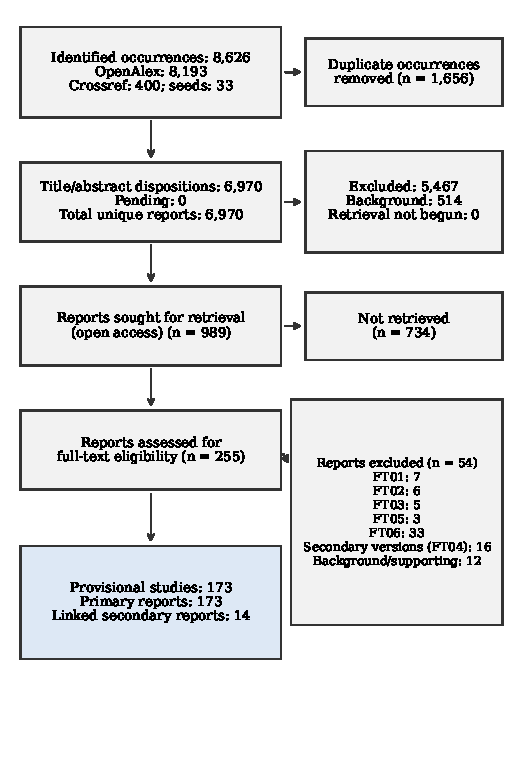
\includegraphics[width=\columnwidth]{fig_flow.pdf}
\caption{Selection flow adapted from PRISMA-ScR. FT01--FT06: full-text exclusion codes (Table~\ref{tab:eligibility}). Records not retrieved were not excluded; they await retrieval or abstract-level charting.}
\label{fig:flow}
\end{figure}

\subsection{Publication and Study Characteristics}
The evidence is recent: \nRecent{} of \nIncluded{} studies (\pctRecent\%) appeared in 2025--2026 (Fig.~\ref{fig:years}). The 2026 count covers January to October only. Preprints, conference papers and theses are common, reflecting the pace of the field; versions were linked to avoid double counting.

\begin{figure}[t]
\centering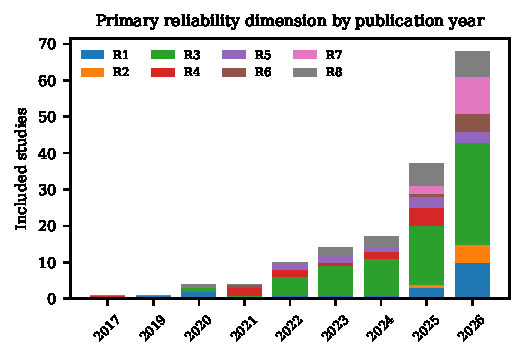
\includegraphics[width=\columnwidth]{fig_years.pdf}
\caption{Included studies by publication year and primary reliability dimension (n = \nIncluded). The 2026 bar covers the search period to October.}
\label{fig:years}
\end{figure}

\subsection{Assets, Contexts, Tasks and Modalities}
Manufactured products dominate (\nManufacturing{} studies), followed by adjacent infrastructure (\nInfra) and energy assets (\nEnergy; Table~\ref{tab:energy}), with \nOther{} in other adjacent settings. Energy studies cover PV modules and PV glass, concentrated solar power receivers, transmission-line insulators, substation infrared sensors, railway catenary components, nuclear plant components, chemical-plant piping, analog gauges and drone inspection of wind and solar assets. RGB imaging dominates. Thermal, EL, X-ray/CT, 3D and multimodal inputs are a minority, and anomaly detection on normal-only training data is the most common task formulation.

% Generated by scripts/make_tables.py
\begin{table*}[t]
\caption{Included studies in energy-asset contexts (n = 21). Dimensions are listed primary first.}
\label{tab:energy}
\centering\scriptsize
\begin{tabularx}{\textwidth}{p{0.07\textwidth}p{0.17\textwidth}p{0.11\textwidth}p{0.08\textwidth}Yp{0.11\textwidth}}
\toprule
Study & Asset/context & Modality & Dimensions & Reliability mechanism (as reported) & Maturity \\
\midrule
\cite{nash2022deep} & Steel/alloy corrosion on assets & RGB & R1; R3 & Bayesian variants of HRNetV2 giving aleatoric and epistemic pixel uncertainty & Industrial dataset (offline) \\
\cite{alqahtani2026robust} & PV modules & RGB PV panel images & R1; R2; R8 & MC-dropout uncertainty with learned-threshold abstention routing ambiguous samples to inspecto... & Benchmark (public) \\
\cite{khandagale2026dasformer} & PV module manufacturing/inspection & EL/visual PV images & R1; R3 & MC-dropout predictive variance and ECE-style calibration loss; variance-based trust threshold & Industrial dataset (offline) \\
\cite{gohel2026interpretable} & Pipeline corrosion/erosion & RGB & R1; R3; R8; R5 & MC-dropout predictive entropy for triage; zero-shot cross-domain tests; leakage-free CV; ultra... & Industrial dataset (offline) \\
\cite{kang2019contact} & Railway catenary contact-wire supports & RGB & R1 & Pixel prediction variance aggregated into image uncertainty to reject blurred images; geometri... & Industrial dataset (offline) \\
\cite{mueez2026vision} & Analog gauges in industrial plants & RGB & R1; R2; R3; R7 & Calibration of numeric correctness, risk-coverage curves, leave-one-dataset-out transfer, corr... & Industrial dataset (offline) \\
\cite{estievenart2025risk} & Concentrated solar power receivers & Thermal-IR & R2; R3; R8 & Risk-control thresholding with finite-sample guarantees on a chosen risk; abstention deferring... & Deployed or operational \\
\cite{mistry2026from} & PV modules & EL and other PV imaging m... & R2; R3; R5; R7 & Risk-coverage selective prediction; robustness to realistic corruptions; reasoning grounded in... & Benchmark (public) \\
\cite{wu2026hdsi} & Transmission-line insulators & RGB & R3; R8; R4 & Cross-dataset generalisation evaluation; split audit revealing scene-level leakage and correct... & Benchmark (public) \\
\cite{he2026self} & PV modules & EL & R3 & Continual self-evolving learning adapting to data shifts and emerging defect categories & Deployed or operational \\
\cite{avramov2026synthetic} & Nuclear power plant components & RGB & R3; R1 & Augmentation versus no augmentation under synthetic-to-real shift; analysis of saturated confi... & Industrial dataset (offline) \\
\cite{bence2026yolov} & PV glass manufacturing & RGB line-scan images & R3; R1 & Domain-balanced sampling and domain consistency objective; evaluation of accuracy and calibrat... & Industrial dataset (offline) \\
\cite{bao2023miad} & Outdoor maintenance inspection & RGB & R3; R8 & Photorealistic MIAD dataset for maintenance inspection under uncontrolled outdoor conditions;... & Benchmark (public) \\
\cite{floreale2025automated} & Power-grid insulator shells & RGB & R5; R7; R8 & Deep SAD on GradCAM/CartoonX explanations flags anomalous explanations for operator reclassifi... & Industrial dataset (offline) \\
\cite{shimbo2023pipe} & External pipe corrosion in chemical plants & RGB & R5 & Expert tacit knowledge converted to annotation criteria; predictions verified by maintenance p... & Deployed or operational \\
\cite{shimbo2023operation} & External pipe corrosion in chemical plants & RGB & R5; R4 & Operational evaluation of the HITL system; subjective visual severity assessment addressed by... & Deployed or operational \\
\cite{amorim2025collaborative} & Solar panel farms & RGB & R5 & Human-in-the-loop mechanism within the decision framework & Benchmark (public) \\
\cite{khandagale2026meta} & PV systems & Multimodal & R6; R1; R3; R5 & Uncertainty gating scales physics priors and modalities when sensors are missing or corrupted;... & Benchmark (public) \\
\cite{hu2025fault} & Substation infrared monitoring sensors & Thermal-IR sensor images & R6 & Classifies infrared-sensor failure modes from sensor outputs & Industrial dataset (offline) \\
\cite{wallace2025inspectvlm} & Drone inspection of wind, solar and property... & RGB; Thermal-IR & R7; R8 & Critical evaluation of unified VLM inspection: grounding, prompt-variability brittleness, dege... & Industrial dataset (offline) \\
\cite{malikussaid2026hybrid} & Wind turbine blades & RGB & R7 & Reports grounded in indexed maintenance procedures; hallucination rate, BLEU-4, ROUGE-L and LL... & Benchmark (public) \\
\bottomrule
\end{tabularx}
\end{table*}


\subsection{Datasets, Partitions and Evaluation Settings}
\nMVTec{} studies use the MVTec AD family and \nVisA{} use VisA. \nRestricted{} rely at least partly on proprietary or restricted data. Code or data release was stated in \nPublicArtifacts{} studies. Threshold-free ranking metrics dominate: AUROC-type metrics appear in \nAUROCEval{} reliability evaluations, against \nCalibEval{} that measure calibration, \nRiskCoverage{} that report risk--coverage or coverage, and \nFalseAlarm{} that report false-alarm rates at an operating point.

\begin{figure}[t]
\centering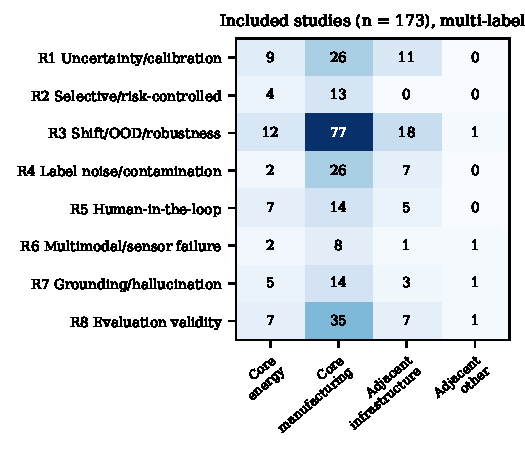
\includegraphics[width=\columnwidth]{fig_evidence.pdf}
\caption{Evidence map: studies addressing each reliability dimension by context (multi-label; n = \nIncluded).}
\label{fig:distribution}
\end{figure}

\section{Results: Reliability Evidence Map}
\label{sec:evidence-map}
Fig.~\ref{fig:distribution} shows the distribution of dimensions across contexts: R3 \nAnyThree, R8 \nAnyEight, R1 \nAnyOne, R4 \nAnyFour, R5 \nAnyFive, R7 \nAnySeven, R2 \nAnyTwo{} and R6 \nAnySix{} studies.

\subsection{Robustness and Distribution Shift (R3)}
Shift is the most studied dimension~\citeThree. Of the R3 studies, \nThreeNatural{} test natural shifts (alone or with synthetic ones) and \nThreeSynthetic{} test synthetic shifts only. Studies with natural shifts consistently report large losses. A crack classifier fell from 94.1\% accuracy on its benchmark to 14.3\% on field images and recovered after fine-tuning on 380 field images~\cite{ndjoko2026automated}. State-of-the-art detectors that saturate MVTec AD degraded under within-category background, illumination and viewpoint shift~\cite{zhang2023industrial,cao2023anomaly}, under robot-captured viewpoints and reflectance~\cite{chang2024rad}, under outdoor maintenance scenes~\cite{bao2023miad} and under railway LiDAR sensor changes~\cite{ghasemlou2026cross}. Corruption benchmarks quantify sensitivity to noise, blur and illumination~\cite{wang2024robustness,cheng2024rad}. Adversarial attacks collapse near-perfect clean scores~\cite{lo2022adversarially,mirzaei2024killing,nafez2025patchguard}, and poisoned training data can make defect inspectors misjudge criticality or miss defects~\cite{johansson2026poisoning}. Mitigations include domain adaptation from laboratory to field~\cite{wang2025efficient,ghoshmondal2025class,oliveirasantos2022domain}, domain generalisation~\cite{trinh2024multiple,chen2022domain}, test-time adaptation~\cite{song2024source,zia2026learning,lei2025adapted}, nuisance filtering and few-shot recalibration of frozen detectors~\cite{cao2026nfad,han2026sparc}, synthetic-to-real training~\cite{cordier2022improving,bondar2025synthetic,tabassum2024adapting,hasan2026xct,avramov2026synthetic}, and continual learning. Continual-learning benchmarks under realistic drift found that dedicated methods rarely beat replay and that geometric drift reduced every method to chance~\cite{weatherly2026rethinking}. Open-set formulations evaluate detection of unseen defect types~\cite{ding2022catching,wang2025distribution,yao2023explicit,liang2026open,alvarez2026foundation,frittoli2022deep}.

\subsection{Uncertainty and Calibration (R1)}
Uncertainty is studied in \nAnyOne{} studies~\citeOne, most often through Monte Carlo dropout, Bayesian layers or ensembles in segmentation and classification~\cite{nash2022deep,kang2019contact,sajedi2020model,liang2020deep,thakur2024deep}. Studies report that epistemic uncertainty rises on OOD images~\cite{nash2022deep} and that uncertainty correlates with misclassification~\cite{sajedi2020model}. Measurement of calibration is less common. Exceptions report expected calibration error for PV defect models~\cite{khandagale2026dasformer}, propose ground-truth-free calibration metrics for manufacturing inspection~\cite{rozanec2023active}, correct overconfident crack classifiers~\cite{chen2025attack}, evaluate calibration on unseen production domains~\cite{bence2026yolov}, and report reliability diagrams and risk--coverage curves for VLM gauge reading on industrial data~\cite{mueez2026vision}. In the last study, high-confidence errors persisted after fine-tuning. Uncertainty of image-derived measurements (corrosion severity, monocular point clouds, super-resolved CT pores) is a distinct strand~\cite{rintrawong2026coverage,malihi2026quantitative,klos2025super}.

\subsection{Decision Policies and Human Inspection Workload (R2, R5)}
Table~\ref{tab:decision} lists the \nGuarFS{} studies with finite-sample guarantees, the \nGuarEOP{} with empirically set operating points, and those evaluated with humans. Finite-sample guarantees take the form of conformal p-values for NDT anomaly detection~\cite{estermann2026unsupervised}, risk-controlled thresholds with expert abstention deployed for months at two CSP plants~\cite{estievenart2025risk}, distribution-free false-alarm tolerance limits~\cite{deng2026distribution}, and exact binomial certificates for selective image restoration~\cite{yang2026saferestore}. Two of these state that coverage does not extend to batch dependence or domain shift~\cite{deng2026distribution,yang2026saferestore}. Empirical policies route high-uncertainty samples to inspectors: rejecting the most uncertain 20\% raised PV fault-classification accuracy from 92.2\% to 97.2\%~\cite{alqahtani2026robust}; reviewing the top 25\% by entropy captured most residual corrosion errors~\cite{gohel2026interpretable}; and a three-way pass/review/reject policy traded workload against error targets~\cite{kinalioglu2026risk}. Human involvement is designed into the workflow in \nHumDes{} studies~\citeHumDes{} and evaluated with humans in \nHumEval~\citeHumEval. These include a preregistered field experiment with factory workers, in which heatmap explanations improved task performance~\cite{senoner2024explainable}; concordance with a certified PV inspector~\cite{mistry2026from}; inter-rater reliability of steel micrograph labels~\cite{durmaz2023microstructure}; inter-operator threshold variance~\cite{mikayilov2025development}; plant operation of a corrosion system~\cite{shimbo2023pipe,shimbo2023operation}; and a field trial of drone-AR bridge inspection~\cite{lapointe2022for}. Review workload was quantified in a few studies, for example 15\% of insulator images flagged for manual reclassification~\cite{floreale2025automated}.

% Generated by scripts/make_tables.py
\begin{table*}[t]
\caption{Studies reporting a decision guarantee or an evaluation with humans (n = 27).}
\label{tab:decision}
\centering\scriptsize
\begin{tabularx}{\textwidth}{p{0.07\textwidth}p{0.17\textwidth}Yp{0.12\textwidth}p{0.12\textwidth}p{0.11\textwidth}}
\toprule
Study & Context & Decision or referral policy (as reported) & Guarantee & Human role & Maturity \\
\midrule
\cite{alqahtani2026robust} & PV modules & Reject if MC-dropout STD above learned threshold; route to human inspectors & Empirical operating point & Designed into workflow & Benchmark (public) \\
\cite{khandagale2026dasformer} & PV module manufacturing/inspection & Conservative policy flags high-variance detections for review & Empirical operating point & Designed into workflow & Industrial dataset (offline) \\
\cite{gohel2026interpretable} & Pipeline corrosion/erosion & Human review of top-25\% entropy & Empirical operating point & Designed into workflow & Industrial dataset (offline) \\
\cite{rozanec2023active} & Shaver logo printing & Products with uncertain score deferred to manual inspection & Empirical operating point & Designed into workflow & Industrial dataset (offline) \\
\cite{sahoo2026hybrid} & Semiconductor wafer maps & Defer low-confidence samples to experts & Empirical operating point & Designed into workflow & Benchmark (public) \\
\cite{thakur2024deep} & Civil structures & PQT rejects outputs whose estimated accuracy is below a threshold; alerts opera... & Empirical operating point & Designed into workflow & Benchmark (public) \\
\cite{kinalioglu2026risk} & Industrial products & Three-way pass/review/reject thresholds from calibration data & Empirical operating point & Designed into workflow & Benchmark (public) \\
\cite{lo2026semantic} & Dynamic industrial inspection via teleo... & VLM invoked below confidence threshold; human confirms safety-critical decisions & Empirical operating point & Designed into workflow & Industrial dataset (offline) \\
\cite{bauer2025handling} & Friction stir welding seams & Confidence threshold defers predictions to manual inspection & Empirical operating point & Designed into workflow & Industrial dataset (offline) \\
\cite{rozanec2022streaming} & Consumer products & Instances above an uncertainty threshold are sent for manual labelling & Empirical operating point & Designed into workflow & Industrial dataset (offline) \\
\cite{mistry2026from} & PV modules & Ambiguous cases escalated to experts & Empirical operating point & Evaluated with humans & Benchmark (public) \\
\cite{mikayilov2025development} & Industrial production lines & Two operating thresholds per model family; operator threshold variance measured & Empirical operating point & Evaluated with humans & Industrial dataset (offline) \\
\cite{hecklerkram2026the} & Manufactured products & Threshold estimated from defect-free data only & Empirical operating point & None & Benchmark (public) \\
\cite{kang2019contact} & Railway catenary contact-wire supports & Image rejected as blurred if uncertainty > mean + 3 SD & Empirical operating point & None & Industrial dataset (offline) \\
\cite{frittoli2022deep} & Silicon wafer production & Novel if score > eta with P = alpha & Empirical operating point & None & Industrial dataset (offline) \\
\cite{jia2026adaptive} & Two-photon lithography microstructures & Batch flagged as novel if votes exceed calibrated threshold & Empirical operating point & None & Industrial dataset (offline) \\
\cite{abbassi2024trimming} & Manufacturing inspection & Inputs below calibrated confidence threshold or out of distribution rejected fr... & Empirical operating point & None & Industrial dataset (offline) \\
\cite{mueez2026vision} & Analog gauges in industrial plants & Proposed safeguards not validated & Empirical operating point & Recommended only & Industrial dataset (offline) \\
\cite{estievenart2025risk} & Concentrated solar power receivers & Risk-controlled threshold with abstention band to domain experts & Finite-sample & Designed into workflow & Deployed or operational \\
\cite{yang2026saferestore} & Industrial SEM inspection images and Ko... & Gate chosen on tuning data, certified on disjoint sample; review option & Finite-sample & Designed into workflow & Benchmark (public) \\
\cite{estermann2026unsupervised} & Industrial NDT components & Flag if p-value < 0.02 & Finite-sample & None & Industrial dataset (offline) \\
\cite{deng2026distribution} & Industrial surface inspection & Tolerance-limit threshold with P >= 1-delta & Finite-sample & None & Benchmark (public) \\
\cite{senoner2024explainable} & Electronics factory quality inspection & Humans approve or reject with AI score; no automated referral & None & Evaluated with humans & Human-subject experiment \\
\cite{durmaz2023microstructure} & Steel microstructure quality control & Thresholds confidential & None & Evaluated with humans & Industrial dataset (offline) \\
\cite{shimbo2023pipe} & External pipe corrosion in chemical pla... & Personnel verify AI predictions & None & Evaluated with humans & Deployed or operational \\
\cite{shimbo2023operation} & External pipe corrosion in chemical pla... & Maintenance personnel verify outputs; high-risk-rank model planned & None & Evaluated with humans & Deployed or operational \\
\cite{lapointe2022for} & Bridge overpasses & Inspector interprets AI detections via AR & None & Evaluated with humans & Field validation \\
\bottomrule
\end{tabularx}
\end{table*}


\subsection{Label Noise and Training Contamination (R4)}
R4 evidence~\citeFour{} mostly injects anomalies into normal-only training sets at controlled rates~\cite{aqeel2025self,das2025adaptive,wang2025softpatch,tan2021trustmae,moradi2025rddpm,aqeel2025robust}. Fewer studies examine naturally occurring label problems: inconsistent labels of suspicious regions~\cite{niu2024learning}, noisy multi-label reports from historical sewer CCTV databases~\cite{chelouche2025when}, low inter-rater agreement in metallography~\cite{durmaz2023microstructure}, and a consensus contamination audit that changed model rankings on a manufacturing dataset~\cite{szklarzewski2026from}.

\subsection{Multimodal Reliability and Sensor Failures (R6)}
Sensor-failure evidence is sparse~\citeSix. Missing-modality tests show that a perturbation curriculum raised welding-defect macro-F1 by 21.5 points when modalities were dropped~\cite{hoang2026supervised}, that removing 3D input cost 4.6 points of image AUROC in RGB--3D detection~\cite{deng2026maf}, and that uncertainty gating degrades gracefully when PV sensor modalities are missing~\cite{khandagale2026meta}. One energy study diagnoses failures of substation infrared sensors themselves~\cite{hu2025fault}. Others compensate failing vision with tactile or event sensing~\cite{jiang2021vision,shi2026industrial} or filter weld-pool disturbances~\cite{cao2026robust}.

\subsection{Evidence Grounding and Traceability (R7)}
Grounding evidence~\citeSeven{} is largely recent and VLM-based (\nVLM{} studies use foundation or vision-language models). Evaluations of general VLMs report weak grounding. A unified VLM for drone inspection of wind and solar assets underperformed task-specific models and defaulted to memorised answers~\cite{wallace2025inspectvlm}. Zero-shot multimodal models reached F1 of about 0.42 on building-defect perception~\cite{zhong2026can}, and VLMs grounded aerial road damage poorly~\cite{liu2026wildroadbench}. Retrieval-augmented and tool-grounded designs reduce hallucination in maintenance reports for wind-turbine blades~\cite{malikussaid2026hybrid}, additive-manufacturing anomaly classification~\cite{naghavikhanghah2025multimodal}, X-ray NDT~\cite{liu2026insightx} and cross-domain anomaly detection~\cite{jiang2026anomalyclaw,deng2026global,chen2026zsg}. Hallucination also arises in reconstruction, where it was assessed for super-resolved CT of lattice defects~\cite{klos2025super}.

\subsection{Evaluation Validity and Validation Maturity (R8)}
R8 studies~\citeEight{} document the gap between benchmarks and inspection. Saturation motivates new benchmarks: state-of-the-art methods score below 60\% AU-PRO on MVTec AD~2~\cite{hecklerkram2026the}, the best challenge entry reached about 57\% segmentation F1 on held-out data~\cite{hecklerkram2026detecting}, and rankings shift on real-world and same-sort datasets~\cite{wang2024real,wang2025hss,baitieva2025beyond,xie2024iad,hecklerkram2025from}. Leakage inflates results: a split audit found 41.7\% of test images sharing source scenes with training~\cite{wu2026hdsi}, and documentation-derived datasets contain repeated views and annotation errors~\cite{bartczak2026dataset}. Low damage prevalence makes most positive alerts false even for accurate classifiers~\cite{plevris2025assessing}. Probability-of-detection curves link AI crack detection to engineering inspection reliability~\cite{kompanets2026evaluation}. Clever Hans strategies go undetected by standard validation~\cite{kauffmann2025explainable,kauffmann2020the,posadamoreno2023scale}, and model selection without labelled anomalies is itself unreliable~\cite{fung2025model,yoo2023dsv}. Validation maturity is low (Fig.~\ref{fig:coverage}): \nBench{} studies rely on public benchmarks, \nIndOffline{} on offline industrial data, \nField{} on field validation~\citeField{} and \nDeployed{} on deployed or operational use~\citeDeployed; \nHumanExp{} is a human-subject experiment.

\begin{figure}[t]
\centering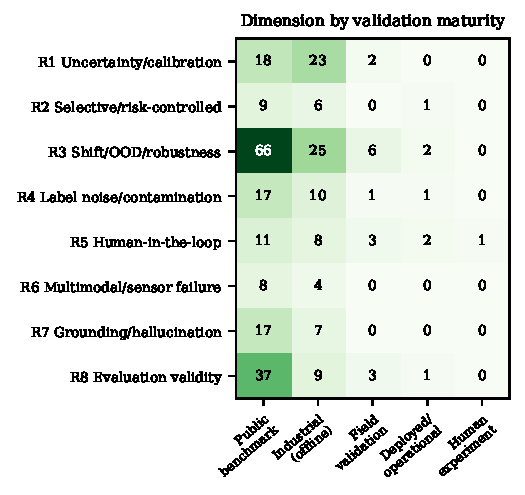
\includegraphics[width=\columnwidth]{fig_maturity.pdf}
\caption{Coverage matrix: studies by reliability dimension (multi-label) and validation maturity (n = \nIncluded). Zero cells mean no included study; they do not establish absence of such evidence in unretrieved reports.}
\label{fig:coverage}
\end{figure}

\section{Discussion}
\label{sec:discussion}

\subsection{Answers to the Review Questions}
RQ1: reliability evidence is concentrated on RGB anomaly detection for manufactured products. Energy-asset studies (\nEnergy) are few and mostly offline, the main exceptions being operational studies in CSP plants, PV EL inspection and chemical-plant piping~\cite{estievenart2025risk,he2026self,shimbo2023pipe,shimbo2023operation}. RQ2: robustness to shift dominates. Uncertainty is often estimated but seldom calibrated or linked to decisions, and sensor failure and grounding are emerging. RQ3: most studies stop at a score. Thresholds are rarely principled, only \nGuarFS{} provide finite-sample guarantees, and human review is mostly recommended rather than evaluated. RQ4: validation is mostly benchmark-based. Studies with natural shifts, field data or audits repeatedly show that benchmark performance overstates inspection reliability.

\subsection{Cross-Cutting Patterns}
Reading the map along the inspection chain (acquisition, model score, decision, human action) shows evidence thinning at each step. Acquisition and model-level robustness (R3, R6) are studied most. Score-level uncertainty (R1) is common but rarely calibrated. Decision-level guarantees (R2) and human-level evaluation (R5) are rare, and they are almost absent under natural shift and in energy settings. This interpretation is ours, derived from the coverage counts. It is consistent with the R8 studies showing that threshold-free metrics, saturated benchmarks and leakage hide decision-relevant errors~\cite{hecklerkram2026the,wu2026hdsi,plevris2025assessing,deng2026distribution}.

\subsection{Implications for Energy and Industrial Inspection}
For practitioners, the evidence argues for evaluating at the decision level: report false-alarm and miss rates at the operating point, calibrate on data resembling the target site, define referral policies and measure the review workload they create, and validate on natural shifts from the target fleet before relying on benchmark results. Guarantees reported in the literature assume exchangeable calibration data~\cite{deng2026distribution,yang2026saferestore}; they need recalibration or monitoring when sites, seasons or sensors change. Image-based findings should remain linked to physical verification (for example ultrasonic thickness or probability-of-detection studies~\cite{rintrawong2026coverage,kompanets2026evaluation}) before maintenance or fitness-for-service conclusions are drawn.

\subsection{Research Opportunities and Their Evidential Basis}
Table~\ref{tab:opportunities} lists opportunities that follow from documented patterns, each with its closest existing work. Sparse cells in the map are not proof of novelty: the \nNotRetrieved{} unretrieved reports and the single-index search may hide relevant studies.

\begin{table*}[t]
\caption{Evidence-grounded research opportunities.}
\label{tab:opportunities}
\centering\footnotesize
\begin{tabularx}{\textwidth}{YYYYY}
\toprule
Observed pattern & Closest work & Question & Required data/evaluation & Qualification \\
\midrule
Finite-sample guarantees are rare and assume exchangeability & \cite{estievenart2025risk,deng2026distribution,yang2026saferestore,estermann2026unsupervised} & Do risk-controlled thresholds keep their coverage under natural site and season shift in energy inspection? & Multi-site data with natural shift; coverage and false-alarm audit over time & Guarantees may need shift-aware or online recalibration \\
Referral is recommended more than evaluated & \cite{kinalioglu2026risk,alqahtani2026robust,senoner2024explainable,floreale2025automated} & What referral policy minimises missed defects for a fixed inspector workload? & Inspector studies with measured workload, time and error & Human studies are costly; simulation is weaker evidence \\
Sensor failure tested mostly synthetically & \cite{hoang2026supervised,deng2026maf,khandagale2026meta,hu2025fault} & How do RGB--thermal UAV inspection models behave with real sensor degradation? & Field data with logged sensor faults; missing-modality tests & Needs operator data access \\
VLM grounding is weak and rarely validated against standards & \cite{wallace2025inspectvlm,malikussaid2026hybrid,mistry2026from,zhong2026can} & Can grounded VLM reports be verified against inspection standards and expert findings? & Expert-annotated reports; hallucination and faithfulness metrics & Rapidly moving model base \\
Benchmarks hide decision errors & \cite{hecklerkram2026the,wu2026hdsi,plevris2025assessing,kompanets2026evaluation} & Which evaluation protocol predicts field reliability of visual inspection? & Leakage-free splits, operating-point metrics, PoD, field follow-up & Requires shared field datasets \\
\bottomrule
\end{tabularx}
\end{table*}

\subsection{Limitations of the Available Evidence}
Most evidence comes from public benchmarks with controlled acquisition and synthetic shifts or contamination. Proprietary data limit reproducibility in industrial studies. Metrics are heterogeneous and mostly threshold-free, which prevents quantitative comparison. Several studies are preprints or appear in venues outside the field. They were charted as reported, with no quality weighting.

\subsection{Limitations of the Review Process}
\label{sec:limits-process}
First, the search used a single bibliographic index; seven of ten known primary studies were retrieved by the original search. Citation tracing has since been integrated but \nPendingTA{} reports still await title/abstract disposition and \nAwaitingRetrieval{} screened reports await retrieval initiation. Second, full texts were retrieved only from open-access locations. \nNotRetrieved{} of \nSought{} reports (largely IEEE, Elsevier and Springer) are not retrieved and not charted from full text, which may bias the map toward open preprints and journals. An exploratory summary of screening rationales covers \nTier{} unretrieved reports with a captured abstract; \nTierTitleOnly{} others lack captured abstracts. This is a report-level retrieval-gap inventory, not independent full-text charting or a test of retrieval bias. Reliability dimensions were extracted from prior screening rationales; energy-title keywords are not interchangeable with the full-text context coding. It cannot establish that missing reports would leave the evidence map unchanged. Third, selection and charting were performed by an AI assistant under the first author's delegation, with one reviewer per decision. A second pass by the same AI assistant over the audit sample revised \nAuditRevised{} decisions (Section~\ref{sec:selection}). It is a consistency check, not the independent human audit the protocol requires, which Daniel subsequently confirmed for the fixed 658-record sample, with agreement on all current decisions. This verification does not constitute independent dual human screening, and an updated sample remains necessary after outstanding selection. Fourth, full texts in languages other than English were excluded (\nExFTFive{} reports). Fifth, the window closes in October 2026, during a period of fast growth; recent preprints may change after peer review.
\authorinput{update this subsection after further screening, manual retrieval and citation tracing; refresh the audit sample for changed decisions.}

\section{Conclusion}
\label{sec:conclusion}
Within the \nIncluded{} studies provisionally assessed to date, reliability research on AI-based visual inspection has expanded rapidly but remains centred on model-level robustness evaluated on public manufacturing benchmarks. Decision-level evidence is scarce: few studies give guarantees, measure referral workload, test real sensor failures or validate in the field, especially for energy assets. Where realistic evaluation is done, it repeatedly shows that benchmark scores overstate inspection reliability. These observations motivate decision-level evaluation under natural shift, with explicit operating points, referral policies and field validation. They remain provisional until the outstanding search additions are screened and any resulting new or revised decisions are covered by an updated human audit.

\section*{Acknowledgment}
No funding was received for this work. \authorinput{acknowledgments, if any.}

\section*{Declarations and Research Artifacts}
\subsection*{Data and Code Availability}
Protocol, search queries and raw responses, decision records, linkage, retrieval logs, charting data, and scripts are available in the project repository (https://github.com/Engr-Daniel/trustworthy-ai-energy). The provisional source snapshot is commit \href{https://github.com/Engr-Daniel/trustworthy-ai-energy/commit/16ec7db16ad56028bf54f69eeb83b2dc1056ca5f}{16ec7db}; the final audited release remains pending. Copyrighted full texts are not redistributed.
\subsection*{Funding and Conflicts of Interest}
This research received no external funding. \authorinput{confirm the conflict-of-interest declaration; no funding does not establish absence of competing interests.}
\subsection*{Author Contributions and AI Assistance}
D.~Oyewale conceived the review, set the protocol, assessed the calibration sample and delegated selection and charting. An AI assistant (Claude, Anthropic) performed the earlier searches, screening, full-text eligibility, charting and drafting under that delegation, with recorded rationales and locators. On 2 November, an OpenAI assistant reconciled saved decision packets, checked derived counts and revised the provisional draft. This reconciliation was not an independent second eligibility review. Also on 2 November, Claude re-examined the \nAuditRows{}-record audit sample and checked every reference against its DOI or arXiv record; this second AI pass is not the human verification audit. D.~Oyewale confirmed human verification of all 658 sampled current decisions on 2 November 2026. AI assistants are not authors.

\appendices
\section{Complete Search Strategies}
\label{app:search}
Exact OpenAlex query strings, fields, filters, pagination and per-page checksums are in \path{review-paper/search-strategy/openalex-queries.json} and \path{runs/OPENALEX-20261022-0[12]/search_manifest.json}; failed and superseded runs (\path{OPENALEX-20261016-01}--\path{03}), the Crossref pilot and seed metadata are in the same location, and \path{corpus/search-runs.csv} lists every run.

\section{Charting Codebook and Decision Rules}
\label{app:codebook}
The charting form (versions 0.1 and 0.2), screening notes 1--14, reason codes and the R1--R8 definitions are in \path{review-paper/charting/charting-form.md}, \path{screening/ta-ai-20261022/screening-notes.md} and \path{screening/reason-codes.csv}; charted values with page locators are in \path{charting/charting.csv}.

\section{Reporting Checklist and Supplementary Evidence}
\label{app:reporting}
\authorinput{complete the PRISMA-ScR checklist with final page numbers after typesetting.} Full inclusion and exclusion records with rationales are in \path{screening/confirmed-decisions.csv}; reports not retrieved are listed in \path{fulltext/not-retrieved.csv}.

\ifreferencesready
  \bibliographystyle{IEEEtran}
  \bibliography{refrence}
\fi

\end{document}
